
\chapter{Waves on a Sloping Beach: Full Theory}\label{chap7}

WE\pageoriginale NOW USE the full theory to consider some of the problems treated by the shallow water theory in Chapter \ref{chap5}, and obtain important modifications and extensions. These problems are considerably more complicated in the full theory and we shall consider only the linearized approximation. As described in Chapter \ref{chap6} we have to solve the following problem for the velocity potential:
\begin{align}
\nabla^2\phi &=0\quad\text{in the fluid},\tag{7.1}\label{chap7:eq7.1}\\
\frac{\partial\phi}{\partial n} &=0\quad\text{on bottom}, \tag{7.2}\label{chap7:eq7.2}\\
\phi_y&+\frac{1}{g}\phi_{tt}=0\quad\text{on}\quad y=0.\tag{7.3}\label{chap7:eq7.3}
\end{align}

Then the surface elevation is given by 
\begin{equation}
\eta= -\frac{1}{g}\left[\phi_t\right]_{y=0}.\tag{7.4}\label{chap7:eq7.4}
\end{equation}

\section{Normal incidence}\label{chap7:sec7.1}

With $x$ out to sea, $y$ vertical, and beach angle $\beta$, we have 
\begin{equation}
\phi_{xx}+\phi_{yy}=0,\tag{7.5}\label{chap7:eq7.5}
\end{equation}
with the boundary conditions.

At the bottom:
\begin{equation}
x\sin\beta +y\cos\beta =0:\frac{\partial\phi}{\partial n}=\phi_x\sin\beta + \phi_y\cos\beta =0.\tag{7.6}\label{chap7:eq7.6}
\end{equation}

On the top $y=0$:
\begin{equation}
\phi_{tt}+g\phi_y=0.\tag{7.7}\label{chap7:eq7.7}
\end{equation}\pageoriginale

If $\phi(x,y,t)$ is of the form
$$
\phi(x,y,t)=S(x,y)e^{-i\omega t},
$$
then \eqref{chap7:eq7.5}-\eqref{chap7:eq7.7} become
\begin{align}
& S_{xx}+S_{yy}=0,\tag{7.8}\label{chap7:eq7.8}\\
\text{Bottom:}\quad & S_x\sin\beta+S_y\cos\beta =0,\tag{7.9}\label{chap7:eq7.9}\\
\text{on}\quad & x\sin\beta+y\cos\beta =0,\notag\\
\text{Top:}\quad & S_y-\ell S=0\quad\text{on}\quad y=0, \tag{7.10}\label{chap7:eq7.10}
\end{align}
where
$$
\ell =\frac{\omega^2}{g}.
$$
\begin{figure}[H]
\centering
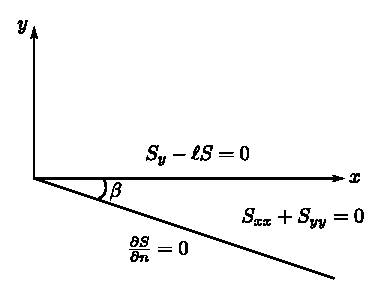
\includegraphics{figures/fig61-7.1.eps}
\caption{}
\label{chap1:fig7.1}
\end{figure}


Hanson in 1926 observed that when $\beta=\frac{\pi}{2N}$ ($N$ is an integer) an exact solution of the problem can be given as the sum of exponentials. For example in the special case $\beta=\frac{\pi}{4},(N=2)$, he obtained
\begin{equation}
\begin{aligned}
S&=\frac{1}{4}(1+i)e^{i\ell x+\ell y}+\frac{1}{4}(1+i)e^{-\ell x-i\ell y},\\
&+\frac{1}{4}(1+i)e^{-i\ell x+\ell y}+\frac{1}{4}(1-i)e^{-\ell x+i\ell y}.
\end{aligned}\tag{7.11}\label{chap7:eq7.11}
\end{equation}\pageoriginale

The first and third terms are just deep water solutions, representing outgoing and incoming waves, respectively, but ignoring the bottom boundary condition \eqref{chap7:eq7.9}. The second and fourth terms correct for the boundary condition and tend to zero as $x\to\infty$ away from the shore. We note that the solution is regular at the shore, with perfect reflection. Thus it corresponds to the $J_0$ solution of \eqref{chap5:eq5.16}. This time we see that the amplitude at infinity is non-zero. The ratio of the amplitude at infinity (combined incident plus reflected) to the total amplitude at the shoreline is 
\begin{equation}
\frac{a_\infty}{a_0}=\frac{1}{\sqrt{2}}.\tag{7.12}\label{chap7:eq7.12}
\end{equation}

In the 1940's Lewy and Stoker (see \cite{key10}) found a consistent way to generate these solutions for the special angles $\beta =\pi/2N$ (and later for $\beta =M\pi/2N$). As $N$ increases, for small beach angles $\beta$, the number of exponentials becomes large. Asymptotics and various quesions for $\beta\ll 1$ become difficult with these formulas. However, Friedrichs \cite{key12} found a form which is useful for these and other purposes. The derivation is not given in the paper. It seems intirely possible that Friedrichs noted that sums of exponentials would follow from complex integrals of the form 
$$
\frac{1}{2\pi i}\int\limits_Cf(\zeta)e^{\zeta(x\pm iy)}\,d\zeta
$$\pageoriginale
when $f(\zeta)$ is a meromorplic function, and observed which factors in $f$ are needed to give the known results. For example it is easy to construct \eqref{chap7:eq7.11} with poles at $\zeta=\pm i\ell$. Here, we give an independent derivation, which is independent of previously known results.

First, by separation of variables, elementary solutions of Laplace's equation are 
\begin{equation}
e^{\zeta x}.e^{\pm i\zeta y}\tag{7.13}\label{chap7:eq7.13}
\end{equation}
and by superposition we obtain a general solution of the equation in \eqref{chap7:eq7.8} to be 
\begin{equation}
S(x,y)=\frac{1}{4\pi i}\int\limits_{\mathscr{C}}f(\zeta)e^{\zeta(x+iy)}\,d\zeta+ \frac{1}{4\pi i}\int\limits_{\mathscr{C}}g(\zeta)e^{\zeta(x-iy)}\,d\zeta \tag{7.14}\label{chap7:eq7.14}
\end{equation}
where $\mathscr{C}$ is a contour in the complex plane to be chosen later. The form \eqref{chap7:eq7.14} is also immediately suggested by the fact that analytic functions of $x+iy$ or $x-iy$ satisfy Laplace's equation. If \eqref{chap7:eq7.14} satisfies the top boundary condition \eqref{chap7:eq7.10} then 
$$
\frac{1}{4\pi i}\int\limits_{\mathscr{C}}\left\{(i\zeta -\ell)f(\zeta)-(i\zeta +\ell)g(\zeta)\right\}e^{\zeta x}\,d\zeta =0.
$$

Since this is true for all $x$, we obtain
\begin{equation}
g(\zeta)=\frac{\zeta +i\ell}{\zeta - i\ell}f(\zeta). \tag{7.15}\label{chap7:eq7.15}
\end{equation}

In order to find out the functional relation between $f$ and $g$ so that \eqref{chap7:eq7.14} satisfies the bottom boundary condition \eqref{chap7:eq7.9}, it\pageoriginale is convenient to introduce polar coordinates. Then on the bottom,
$$
x=r\cos\beta,\; y= -r\sin\beta,
$$
the boundary condition \eqref{chap7:eq7.9} is satisfied by \eqref{chap7:eq7.14} if 
\begin{align*}
&\frac{1}{4\pi i}\int\limits_{\mathscr{C}}(\sin\beta +i\cos\beta)\zeta e^{\zeta re^{-i\beta}}f(\zeta)\,d\zeta\\
&\qquad +\frac{1}{4\pi i}\int\limits_{\mathscr{C}}(\sin\beta-i\cos\beta)\zeta e^{\zeta re^{i\beta}}g(\zeta)\,d\zeta =0,\\
\text{\ie}\quad& \frac{1}{4\pi}\int\limits_{\mathscr{C}}e^{-i\beta}\zeta e^{\zeta re^{-i\beta}}f(\zeta)\,d\zeta -\frac{1}{4\pi}\int\limits_{\mathscr{C}}e^{i\beta} \zeta e^{\zeta re^{i\beta}}f(\zeta)\,d\zeta =0.
\end{align*}

Using the transformation $\zeta =\zeta' e^{2i\beta}$ for the first integral, we obtain
\begin{equation}
\frac{1}{4\pi}\int\limits_{\mathscr{C'}}e^{2i\beta}\zeta'e^{\zeta're^{i\beta}}f\left(\zeta' e^{2i\beta}\right)\,d\zeta'-\frac{1}{4\pi}\int\limits_{\mathscr{C}}\zeta e^{\zeta re^{i\beta}}g(\zeta)\,d\zeta =0.\tag{7.16}\label{chap7:eq7.16}
\end{equation}
where $\mathscr{C'}$ is the image of $\mathscr{C}$ under the map $\zeta\to \zeta'e^{2i\beta}$.

If $\mathscr{C'}$ can be deformed back to $\mathscr{C}$ without crossing singularities then \eqref{chap7:eq7.16} can be replaced by 
$$
\frac{1}{4\pi}\int\limits_{\mathscr{C}} \left[ f\left(\zeta e^{2i\beta}\right) e^{2i\beta} - g(\zeta)\right]\zeta e^{\zeta re^{i\beta}}\, d\zeta =0.
$$

This gives
\begin{equation}
g(\zeta) = e^{2i\beta} f \left(\zeta e^{2i\beta} \right).\tag{7.17}\label{chap7:eq7.17}
\end{equation}

If we combine \eqref{chap7:eq7.15} and \eqref{chap7:eq7.17} we have the functional relation
\begin{equation}
f(\zeta)=e^{2i\beta}\frac{\zeta-i\ell}{\zeta+i\ell}f\left(\zeta e^{2i\beta}\right)\tag{7.18}\label{chap7:eq7.18}
\end{equation}
for $f(\zeta)$. 

\subsection*{\bf Special case $\beta =\pi/2N$}.\pageoriginale

It will be convenient in this case, to define $w$ as 
\begin{equation}
w=e^{2i\beta}=e^{\pi i/N}\tag{7.19}\label{chap7:eq7.19}
\end{equation}
with the properties
\begin{equation}
w^N=-1,\;w^{2N}=1.\tag{7.20}\label{chap7:eq7.20}
\end{equation}

Then \eqref{chap7:eq7.18} becomes
\begin{equation}
f(\zeta)=\frac{\zeta-i\ell}{\zeta+i\ell}wf(w\zeta). \tag{7.21}\label{chap7:eq7.21}
\end{equation}

If this relation is applied $2N$ times to relate $f(\zeta)$ to $f(w^{2N}\zeta)$ the accumulated factors cancel and we deduce only that $f(\zeta)$ is single-valued. If we apply it $N$ times to relate $f(\zeta)$ to $f(w^N\zeta)$, we have 
\begin{equation}
f(\zeta)= -\frac{(\zeta-i\ell)\,(w\zeta-i\ell)\ldots \left(w^{N-1}\zeta-i\ell \right)}{(\zeta+i\ell)\,(w\zeta+i\ell)\ldots\left(w^{N-1}\zeta+i\ell\right)} f(-\zeta),\tag{7.22}\label{chap7:eq7.22}
\end{equation}
since $w^N= -1$. In the multiplying function, we observe that the numerator $\mathscr{N}(\zeta)=(-1)^N\mathscr{D}(-\zeta)$ where $\mathscr{D}(\zeta)$ is the denominator, so that solutions for $f(\zeta)$ are easily read off. First it is convenient to modify \eqref{chap7:eq7.22} to 
\begin{equation}
f(\zeta)= -\frac{(\zeta+i\ell w)\,(\zeta+i\ell w^2)\ldots\left(\zeta+i\ell w^N\right)}{(\zeta-i\ell w)\,(\zeta-i\ell w^2)\ldots\left(\zeta-i\ell w^N\right)}f(-\zeta),\tag{7.23}\label{chap7:eq7.23}
\end{equation}
by taking out factors in $w$, using
$$
w^{-m}= -w^{N-m}
$$
and re-ordering. We then observe that 
\begin{equation}
f(\zeta)=\frac{\zeta^{N-1}}{(\zeta-i\ell w)\,(\zeta-i\ell w^2)\ldots\left(\zeta- i\ell w^N\right)}\tag{7.24}\label{chap7:eq7.24}
\end{equation}\pageoriginale
is a solution, the factor $\zeta^{N-1}$ (or some equivalent) being necessary to adjust the spare powers of $-1$. We check that this not only satisfies \eqref{chap7:eq7.23}, but also the original \eqref{chap7:eq7.21}. We show that this leads to a satisfactory solution for $S(x,y)$ and then return to consider its uniqueness.

We introduce
\begin{align}
& \zeta_n=i\ell w^n=i\ell e^{n\pi i/N},\tag{7.25}\label{chap7:eq7.25}\\
\intertext{and write}
& f(\zeta)=\frac{\zeta^{N-1}}{\left(\zeta-\zeta_1\right)\ldots\left(\zeta- \zeta_N\right)}.\tag{7.26}\label{chap7:eq7.26}
\end{align}

Then, from \eqref{chap7:eq7.15},
\begin{equation}
g(\zeta)=\frac{\zeta^{N-1}}{\left(\zeta-\zeta_0\right)\ldots\left(\zeta- \zeta_{N-1}\right)}.\tag{7.27}\label{chap7:eq7.27}
\end{equation}

The solution \eqref{chap7:eq7.14} becomes 
{\fontsize{10}{12}\selectfont
\begin{equation}
S(x,y)=\frac{1}{4\pi i}\int\limits_{\mathscr{C}}\frac{\zeta^{N-1}e^{\zeta(x+iy)}} {\left(\zeta-\zeta_1\right)\ldots\left(\zeta-\zeta_N\right)}\,d\zeta+ \frac{1} {4\pi i}\int\limits_{\mathscr{C}}\frac{\zeta^{N-1}e^{\zeta(x-iy)}}{\left(\zeta- \zeta_0 \right)\ldots\left(\zeta-\zeta_{N-1}\right)}\,d\zeta. \tag{7.28}\label{chap7:eq7.28}
\end{equation}}

In particular, on the surface $y=0$, 
\begin{equation}
S(x,0)=\frac{1}{2\pi i}\int\limits_{\mathscr{C}}\frac{\zeta^Ne^{\zeta x}}{\left(\zeta- \zeta_0\right)\ldots\left(\zeta-\zeta_N\right)}\,d\zeta; \tag{7.29}\label{chap7:eq7.29}
\end{equation}
the surface elevation is given by 
\begin{equation}
\eta(x,t)=\frac{i\omega}{g}S(x,0)e^{-i\omega t}.\tag{7.30}\label{chap7:eq7.30}
\end{equation}

\medskip
\noindent{\textbf{Solution regular at the shoreline.}}\pageoriginale

The singularities in \eqref{chap7:eq7.28} are poles at 
$$
\zeta=\zeta_n=i\ell e^{\pi in/N},\;n=0,\ldots,N;
$$
they lie on the semicircle $\mathscr{R}\zeta\leq 0$ shown in Fig. 7.2. If $\mathscr{C}$ is taken to be a contour enclosing all these poles then the important condition following \eqref{chap7:eq7.16} that, after rotation, $\mathscr{C'}$ should be deformable back to $\mathscr{C}$ is satisfied. With this contour, $S(x,y)$ is bounded for all $x$ and $y$, and is regular at the shoreline. In fact expanding the integral as the sum of the residues at the poles we have contributions involving only exponentials $e^{\zeta_n(x\pm iy)}$ 
\begin{figure}[H]
\centering
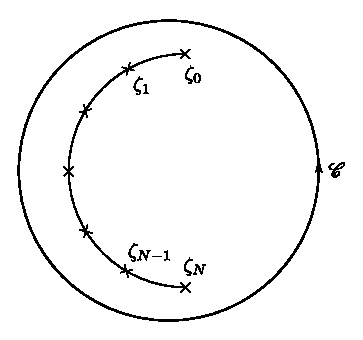
\includegraphics{figures/fig61-7.2.eps}
\caption{}
\label{chap1:fig7.2}
\end{figure}

All these have acceptable behavior as $x\to\infty$ since $\mathscr{R}\zeta_n\leq 0$ for $n=0,1,\ldots,N$. In particular
\begin{equation}
S(x,0)=\sum\limits_0^N c_n e^{\zeta_n x},\tag{7.31}\label{chap7:eq7.31}
\end{equation}
where 
$$
c_n=\frac{\zeta_n^N}{\left(\zeta_n-\zeta_0\right)\ldots\left(\zeta_n-\zeta_N \right)},
$$\pageoriginale
omitting the zero factor in the denominator.

\medskip
\noindent{\textbf{Value at shoreline.}

From \eqref{chap7:eq7.29}
$$
S(0,0)=\frac{1}{2\pi i}\int\limits_{\mathscr{C}}\frac{\zeta^N}{\left(\zeta- \zeta_0\right)\ldots\left(\zeta-\zeta_N\right)}\,d\zeta.
$$

Taking $\mathscr{C}$ to be a large contour and noting that the integrand is $\sim 1/\zeta$ as $\zeta\to\infty$, we have
\begin{equation}
S(0,0)=1.\tag{7.32}\label{chap7:eq7.32}
\end{equation}

Of course any multiple of $S(x,y)$ is also a solution.

\medskip
\noindent{\textbf{Behavior as $x\to\infty$.}}

Since $\mathscr{R}\zeta_n<0$ except for $\zeta_0=i\ell$ and $\zeta_N=-i\ell$, the asymptotic behavior of the solution as $x\to\infty$ is given by the latter. We have, from the residues at $\pm i\ell$, 
\begin{align}
& S(x,y)\sim\frac{1}{2D^*}e^{-i\ell x+\ell y}+\frac{1}{2D}e^{i\ell x+\ell y}, \tag{7.33}\label{chap7:eq7.33}\\
\intertext{where}
& D=(1-w)\,(1-w)\ldots\left(1-w^{N-1}\right),w=e^{\pi i/N}, \tag{7.34}\label{chap7:eq7.34}
\end{align}
and $D^*$ denotes complex conjugate of $D$. This shows the equal amplitude of incoming and outgoing waves; we have perfect reflection. We can also write
\begin{equation}
S(x,0)\sim\frac{1}{|D|}\cos(\ell x-\arg D).\tag{7.35}\label{chap7:eq7.35}
\end{equation}\pageoriginale

\medskip
\noindent{\textbf{The amplitude factor $D$.}

The product $DD^*$ contains all the 2Nth roots of unity except $+1$ and $-1$. Therefore
$$
DD^*=\underset{W\to 1}{\lim}\frac{W^{2N}-1}{(W-1)\,(W+1)}=N.
$$

Moreover,
$$
\frac{D}{D^*}=\frac{(1-w)\ldots\left(1-w^{N-1}\right)}{(1-w^*)\ldots \left(1-  w^{*^{N-1}}\right)}.
$$

But
$$
\frac{1-w^n}{1-w^{*^n}}=\frac{1-w^n}{1-w^{-n}}= -w^n.
$$

Hence 
\begin{align*}
\frac{D}{D^*}  & = (-1)^{N-1} w \cdot w \ldots w^{N-1} = (-1)^{N-1} w^{\frac{N(N-1)}{2}}\\
& = e^{-\pi i(N-1)/2}.
\end{align*}

Therefore
\begin{equation}
D=N^{1/2} e^{-\pi i\frac{N-1}{4}}.\tag{7.36}\label{chap7:eq7.36}
\end{equation}

We note that the ratio of amplitudes is 
\begin{equation}
\frac{a_\infty}{a_0}=\frac{1}{N^{1/2}}=\left(\frac{2\beta}{\pi}\right)^{1/2}. \tag{7.37}\label{chap7:eq7.37}
\end{equation}

Since this holds for a sequence $\beta =\pi/2N$ converging to zero, if $a_\infty/a_0$ is an analytic function of $\beta$, this formula holds for all $\beta$. The formula checks with \eqref{chap7:eq7.12}, and was quoted in the discussion of Section \ref{chap5:sec5.3}. 

\subsection*{\bf Singular solutions}.\pageoriginale

In view of the following conditions on $\mathscr{C}$:
\begin{enumerate}
\item [(a)] After a rotation through $2\beta$ to a new path $\mathscr{C'},\mathscr{C'}$ must be deformable back to the original $\mathscr{C}$ without crossing a singularity;
\item [(b)] A path going to $\infty$ must have $\mathscr{R}\zeta <0$ as $\zeta\to\infty$, in order that the integrals in \eqref{chap7:eq7.28} be convergent for $x>0$;
\end{enumerate}
the only other choices of contour are $\mathscr{C}_1$ or $\mathscr{C}_2$, shown in Fig. 7.3, or some combination. 
\begin{figure}[H]
\centering
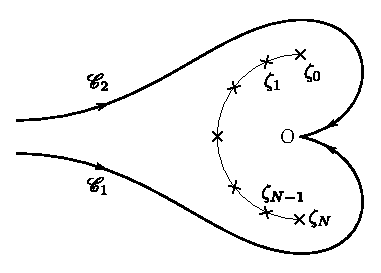
\includegraphics{figures/fig61-7.3.eps}
\caption{}
\label{chap1:fig7.3}
\end{figure}

We consider $S_1(x,0)$ in \eqref{chap7:eq7.29} for the path $\mathscr{C}_1$.

Since the integrand $\sim 1/\zeta$ as $\zeta\to\infty$, the convergence of the integral is lost when $x=0$. Accordingly $S(x,0)$ is singular at the shoreline. We may write
\begin{align*}
S_1(x,0) &= \frac{1}{2\pi i}\int\limits_{-\infty}^A\frac{e^{\zeta x}}{\zeta}\,d\zeta+0(1),\; x\to 0\\
& =\frac{1}{2\pi i}\int\limits_{AX}^\infty e^{-\xi}\frac{d\xi}{\xi}+ 0 \; (1), \quad\text{where}\quad\zeta = -\frac{\xi}{x}\\
&=\frac{1}{2\pi i}\int\limits_{Ax}^1\frac{d\xi}{\xi}+0(1),\\
&= -\frac{1}{2\pi i}\log x+0(1),\tag{7.38}\label{chap7:eq7.38}
\end{align*}\pageoriginale
so the singularity is logarithmic.

We may also use partial fractions and write
\begin{align*}
S_1(x,0) &= \sum\limits_{n=0}^N c_n\frac{1}{2\pi i}\int\limits_{\mathscr{C}_1} \frac{e^{\zeta x}}{\zeta-\zeta_n}\,d\zeta\\
&= \sum\limits_{\mathfrak{J}\zeta_n\leq 0}c_n e^{\zeta_nx}+\sum\limits_{\mathfrak{J} \zeta_n >0}c_n\frac{1}{2\pi i}\int\limits_{-\infty}^0 \frac{e^{\zeta x}}{\zeta-\zeta_n} \,d\zeta.\tag{7.39}\label{chap7:eq7.39}
\end{align*}

(The latter integral is indented above the pole at $\zeta_{N/2}$ in the case $N$ is even). The transformation $\zeta=\zeta_n-\zeta/x$ converts the final integrals into standard exponential integrals.

As $x\to\infty$, the dominant term in \eqref{chap7:eq7.39} is from the pole at $\zeta_N=-i\ell$. Therefore,
\begin{equation}
S_1(x,0)\sim c_N e^{-i\ell x},\;x\to\infty.\tag{7.40}\label{chap7:eq7.40}
\end{equation}

Thus $S_1(x,0)$ represents a purely incoming wave with loss of energy at the beach.

Similarly, if $\mathscr{C}_2$ (Fig. 7.3) is taken in \eqref{chap7:eq7.29}, the corresponding solution $S_2(x,0)$ represents a purely outgoing wave, with logarithmic singularity at the shoreline.

The correspondence with the Bessel functions of the shallow water theory, Section \ref{chap5:sec5.3}, is 
\begin{equation}
\begin{aligned}
S(x,0) =& S_1(x,0)-S_2(x.0)\leftrightarrow J_0,\\
&S_1(x,0)+S_2(x,0)\leftrightarrow -iY_0.
\end{aligned}\tag{7.41}\label{chap7:eq7.41}
\end{equation}

\subsection*{\bf Uniqueness of the solution of the functional relation for $f(\zeta)$}.\pageoriginale

One could show that the uniqueness of the solutions $S(x,y),\break S_1(x,y),
S_2(x,y)$, under the various conditions at $x=0$ and $x\to\infty$, by
direct arguments. However it is interesting to consider the uniqueness
of the solution to the functional equation \eqref{chap7:eq7.21}
directly. This is especially so, since important alternative solutions
arise in the corresponding case for oblique incidence, which we
consider in Section \ref{chap7:sec7.5}. 

If $f(\zeta)$ is set equal to $G(\zeta)$ times the expression in \eqref{chap7:eq7.24} and substituted in \eqref{chap7:eq7.21}, it follows that 
\begin{equation}
G(\zeta)=G(w\zeta),\;w=e^{\pi i/N}.\tag{7.42}\label{chap7:eq7.42}
\end{equation}

Clearly $G(\zeta)=H(\zeta^{2N})$ is a solution for any single valued function $H(z)$. It is also the only solution under reasonable hypotheses.
\begin{proof}
We know that $G(\zeta)$ is single-valued. Suppose that it has a Laurent expansion in some annular region, \ie
\begin{equation}
G(\zeta)=\sum\limits_{-\infty}^\infty a_m\zeta^m.\tag{7.43}\label{chap7:eq7.43}
\end{equation}

Then
\begin{align*}
a_m &= \frac{1}{2\pi i}\oint \frac{G(s)}{s^{m+1}}\,ds\\
&=\frac{1}{2\pi i}\oint\frac{G(wt)}{t^{m+1}}\,dt.\frac{1}{w^m},\;s=wt,\\
&=\frac{1}{2\pi i}\oint\frac{G(t)}{t^{m+1}}\,dt.\frac{1}{w^m},\quad\text{from \eqref{chap7:eq7.42}},\\
&=\frac{a_m}{w^m}
\end{align*}

Therefore\pageoriginale $a_m=0$ unless $m=0,\pm 2N, \pm 4N,\ldots$. Thus from \eqref{chap7:eq7.43}, 
$$
G(\zeta)=H\left(\zeta^{2N}\right)
$$
where $H(z)$ is a single-valued function.

Although the solution of \eqref{chap7:eq7.21} is non-unique to this extent, the extra possibility does not appear to affect $S(x,y)$. We consider the case where $\mathscr{C}$ is a closed contour and include the extra factor $H(\zeta^{2N})$ in \eqref{chap7:eq7.28}. If $H(\zeta^{2N})$ is analytic inside $\mathscr{C}$, the residues at $\zeta_n$ have an extra factor $H(\zeta_n^{2N})$. Since $\zeta_n^{2N}=(i\ell)^{2N}$, this is independent of $n$ and leads only to a constant factor multiplying $S(x,y)$. If $H(z)$ has a pole at the origin, then $H(\zeta^{2N})\propto\zeta^{-m}$ where $m$ is at least $2N$. The residue would lead to positive powers of $x$ and $y$ in $S(x,y)$; these are unacceptable. If $H(z)$ has a pole at $z=A$, then $H(\zeta^{2N})$ has poles at $\zeta=A^{1/2N}$. Some of these have $\mathscr{R}\zeta >0$ and lead to exponentials with positive exponent in $S(x,y)$; again they are unacceptable for a physical solution. 
 \end{proof}

\section{The shallow water approximation}\label{chap7:sec7.2}

Let $\beta\to 0$ in such a manner that $\frac{\ell}{\beta}x$ is fixed and let $\zeta=\frac{\ell}{\beta}\eta$ in \eqref{chap7:eq7.29}. Then 
$$
S(x,0)=\frac{1}{2\pi i}\int\limits_{\mathscr{C}}\frac{e^{\ell x\eta/\beta}\,d\eta} {\eta\left(1-\frac{\beta\zeta_0}{\ell\eta}\right)\ldots\left(1-\frac{\beta\zeta_N}{\ell\eta}\right)}
$$
Now 
\begin{align*}
&\log\left\{\left(1-\frac{\beta\zeta_0}{\ell\eta}\right)\ldots\left(1-\frac {\beta\zeta_N}{\ell\eta}\right)\right\}\\
&\quad=\log\left(1-\frac{\beta\zeta_0}{\ell\eta}\right)+\cdots+\log\left(1- \frac{\beta\zeta_N}{\ell\eta}\right)\\
&\quad =-\frac{\beta}{\ell\eta}\left(\zeta_0+\cdots+\zeta_N\right)+0 (\beta^2N)\\
&\quad =-\frac{i\beta}{\eta}\left(1+w+\cdots+w^N\right)+0(\beta)\\
&\quad =-\frac{i\beta}{\eta}\;\frac{w^{N+1}-1}{w-1}+0(\beta)\\
&\quad =+\frac{i\beta}{\eta}\;\frac{w+1}{w-1}+0(\beta).
\end{align*}\pageoriginale

Since
\begin{align*}
& w=e^{\frac{\pi i}{N}} = 1  + \frac{\pi i}{N}+0\left(\frac{1}{N^2}\right)\\
\intertext{we have}
& \frac{w+1}{w-1}=\frac{2N}{\pi i}+0(\beta).
\end{align*}

Hence 
\begin{equation}
\log\left(1-\frac{\beta\zeta_0}{\ell\eta}\right)\ldots\left(1-\frac{\beta \zeta_N}{\ell\eta}\right)=\frac{1}{\eta}+0(\beta). \tag{7.44}\label{chap7:eq7.44}
\end{equation}

Therefore
\begin{equation}
\begin{aligned}
S(x,0) &\sim \frac{1}{2\pi i}\int\limits_{\mathscr{C}}\frac{\exp\left(\frac{\ell x}{\beta}\eta-\frac{1}{\eta}\right)}{\eta}\,d\eta\\
&= J_0\left(2 \sqrt{\frac{\ell x}{\beta}} \; \right),\;\ell=\frac{\omega^2}{g}. 
\end{aligned}\tag{7.45}\label{chap7:eq7.45}
\end{equation}

This is the solution we obtained in shallow water theory.

Since this is the asymptotic behavior with $\ell x/\beta$ held fixed, it is appropriate only for $x=0(\beta)$. 

\section{Behavior as $\beta\to 0$}\label{chap7:sec7.3}\pageoriginale

Friedrichs \cite{key12} obtained improved approximations for small beach angles. The main step is to improve on the approximation \eqref{chap7:eq7.44}, but we work with different variables. It is convenient to set $\zeta =iz$ in \eqref{chap7:eq7.29} and work with the form 
\begin{equation}
S(x)=\frac{1}{2\pi i}\int\limits_{\mathscr{C}}\frac{z^N e^{izx}} {\left(z-z_0\right)\ldots\left(z-z_N\right)}\,dz,\;z_n=\ell e^{\pi in/N}. \tag{7.46}\label{chap7:eq7.46}
\end{equation}

Now, for large $N$ (small $\beta$),
$$
\frac{1}{2}\log\left(1-\frac{z_0}{z}\right)+\log\left(1-\frac{z_1}{z}\right)+ \cdots+\log\left(1-\frac{z_{N-1}}{z}\right)+\frac{1}{2}\log \left(1-\frac{z_N}{z} \right)
$$
is a Riemann sum approximation to the integral
\begin{equation}
N\int\limits_0^1\log\left(1-\frac{\ell e^{\pi
    i\sigma}}{z}\right)\,d\sigma, \tag{7.47}\label{chap7:eq7.47} 
\end{equation}
taking the dissection $\sigma =n/N$ and $d\sigma =1/N$. If we let this
be\break $2NiF(z)/\pi=iF(z)/\beta$, so that  
\begin{align}
F(z) &= \frac{\pi}{2i}\int\limits_0^1\log\left(1-\frac{\ell e^{\pi i\sigma}}{z} \right)\,d\sigma,\tag{7.48}\label{chap7:eq7.48}\\
\intertext{we have}
S(x) &\sim \frac{1}{2\pi i}\int\limits_{\mathscr{C}}\frac{e^{izx-\frac{i}{\beta} F(z)}}{(z-\ell)^{1/2}(z+\ell)^{1/2}}\,dz.\tag{7.49}\label{chap7:eq7.49}
\end{align}

(Note $z_0=\ell, z_N= -\ell$.)

Expression \eqref{chap7:eq7.49} is valid for small $\beta$, irrespective of $x$. But further approximations can now be made. The shallow water result, for example, corresponds to the approximation
$$
F(z)\sim -\frac{\ell}{z}\quad\text{for large}\quad z.
$$\pageoriginale

The main approximation that Friedrichs considered is the limiting behavior $\beta\to 0$ with the depth $\beta x$ fixed. The precise form is $\ell\beta x$ fixed, but we will not trouble to normalize the variables completely. The exponent in \eqref{chap7:eq7.49} is 
$$
\frac{1}{\beta}(\beta xz-F(z)),
$$
so the saddle point method can be applied for $\beta\to 0$, $\beta x$ fixed. It is convenient first to simplify \eqref{chap7:eq7.48} by the substitution $\tau =ze^{-\pi i\sigma}$ to give
\begin{equation}
F(z)=\frac{1}{2}\int\limits_0^z\frac{1}{\tau}\log \frac{\tau+\ell}{\tau-\ell} \,d.\tag{7.50}\label{chap7:eq7.50}
\end{equation}

Then the saddle points $z=\pm\kappa, \kappa >\ell >0$, satisfy
\begin{align}
\beta x=F'(\kappa) &=\frac{1}{2\kappa}\log \frac{\kappa+\ell}{\kappa-\ell} \tag{7.51}\label{chap7:eq7.51}\\
&= \frac{1}{\kappa}\tan h^{-1}\frac{\ell}{\kappa}. \tag{7.52}\label{chap7:eq7.52}
\end{align}

We note that $\kappa$ is a function of $x$ and \eqref{chap7:eq7.52} can be re-written
\begin{equation}
\ell =\frac{\omega^2}{g}=\kappa\tan h\kappa\beta x. \tag{7.53}\label{chap7:eq7.53}
\end{equation}

This is exactly the relation \eqref{chap6:eq6.34} with $h_0=\beta x$, so that $\kappa(x)$ is the local wave number. This is confirmed in the full saddle point approximation to \eqref{chap7:eq7.49}. We have 
\begin{align}
S(x)&\sim \left(\frac{\beta}{2\pi}\right)^{1/2} \frac{e^{i\theta(x)}} {\left\{ \left(\kappa^2-\ell^2\right)|F''(\kappa)|\right\}^{1/2}} \tag{7.54}\label{chap7:eq7.54}\\
\intertext{where}
& \theta(x)=\kappa x-\frac{1}{\beta}F(\kappa).\tag{7.55}\label{chap7:eq7.55}
\end{align}

Then,\pageoriginale the local wave number discussed in \eqref{chap5:eq5.14} is
$$
\theta_x=\kappa +\left\{x-\frac{1}{\beta}F'(\kappa)\right\}\frac{d\kappa} {dx}=\kappa,
$$
from \eqref{chap7:eq7.51}. So we see that the local wavenumber changes with respect to $x$ according to \eqref{chap7:eq7.53}, this would be expected in advance and has often been used as a direct approximation. The amplitude factor in \eqref{chap7:eq7.54} also has a simple interpretation. It can be shown that it satisfies
\begin{equation}
A^2C(\kappa)=\quad\text{constant},\tag{7.56}\label{chap7:eq7.56}
\end{equation}
where $C(\kappa)$ is the group velocity $\partial\omega/\partial\kappa$. This is a statement of constant energy flux, and again has often been used directly. 

The approximation in \eqref{chap7:eq7.53}-\eqref{chap7:eq7.55} overlaps with the shallow water approximation \eqref{chap7:eq7.45} as $\beta x\to 0$ and gives the correct asymptotic behavior at infinity $(\beta x\to\infty)$. In a typical case of $\beta =6^\circ$, numerical work on the exact solution showed that the shallow water result was good from the shoreline to a distance out of two wavelengths, whereas \eqref{chap7:eq7.53}-\eqref{chap7:eq7.55} applied from about one third of a wavelength out to infinity.

\section{General $\beta$}\label{chap7:sec7.4}

We note that \eqref{chap7:eq7.18} can in fact be solved in terms of an integral for all values of $\beta$. This was obtained by Peters \cite{key13}. The form appears to make it difficult to use in any very practical way, so we just quote the result:
\begin{equation}
\log\left\{\zeta f(\zeta)\right\}=\frac{1}{2\pi i}\int\limits_0^\infty\log\left( \frac{z-i\ell}{z+i\ell}\right).\frac{\pi}{\beta}\;\frac{z^{\frac{\pi}{\beta}-1}} {z^{\pi/\beta}-\zeta^{\pi/\beta}}\,dz\tag{7.57}\label{chap7:eq7.57}
\end{equation}\pageoriginale
in $0<\arg\zeta <2\beta$, with suitable analytic continuation.

\section{Oblique incidence and edge waves}\label{chap7:sec7.5}

We now consider solutions that include dependence on the longshore co-ordinate, which is taken to be $x_2$. These will include waves with oblique incidence at infinity, and edge waves trapped near the shore. In \eqref{chap7:eq7.1}-\eqref{chap7:eq7.3}, we take \footnote{We use $x$ rather than $x_1$ for the offshore coordinate, since it is only $x$ that appears after the separation \eqref{chap7:eq7.58}.}
\begin{gather}
\phi\left(x,x_2,y,t\right)=S(x,y)e^{ikx_2-i\omega t}, \tag{7.58}\label{chap7:eq7.58}\\
\intertext{and the problem for $S(x,y)$ is to solve}
S_{xx}+S_{yy}-k^2S=0,\tag{7.59}\label{chap7:eq7.59}\\
\intertext{with boundary conditions}
\text{Top}\quad y=0:S_y-\lambda S=0,\lambda =\omega^2/g. \tag{7.60}\label{chap7:eq7.60}\\
\text{Bottom}\quad x\sin\beta +y\cos\beta =0:S_x\sin\beta +S_y\cos\beta=0. \tag{7.61}\label{chap7:eq7.61}
\end{gather}

Again Hanson \cite{key11} had found solutions as the sum of exponentials in some special cases $\beta=\pi/2N$. For $\beta =\pi/4$ he had 
\begin{align}
S(x,y) &= \frac{1}{4}\left(1+\frac{i\lambda}{\ell}\right)\left\{e^{i\ell x+\lambda y}+e^{-\lambda x-i\ell y}\right\}+\text{\; complex conjugate} \tag{7.62}\label{chap7:eq7.62}\\
\intertext{with}
\lambda &= \sqrt{\ell^2+k^2},\; 0<\ell <\infty,\; k<\lambda <\infty. \tag{7.63}\label{chap7:eq7.63}
\end{align}

As $x\to\infty$, the asymptotic behavior is given by the first term and its conjugate. Combined with \eqref{chap7:eq7.58}, we have 
\begin{equation}
\begin{aligned}
\phi &\sim\frac{1}{4}\left\{\left(1+\frac{i\lambda}{\ell}\right)e^{i\ell x+ikx_2-i\omega t}\right.\\
&\quad +\left.\left(1-\frac{i\lambda}{\ell}\right)e^{-i\ell x+ikx_2-i\omega t}\right\}e^{\lambda y}.
\end{aligned}\tag{7.64}\label{chap7:eq7.64}
\end{equation}\pageoriginale

This represents an incoming oblique wave travelling in the direction $(-\ell,k)$, and its prefect reflection in the direction $(\ell,k)$. Perfect reflection and regularity at the shore go together as before.

Much earlier Stokes (1846) had found the basic edge wave solution
\begin{equation}
S=e^{-kx\cos\beta+ky\sin\beta},\;\lambda=\frac{\omega^2}{g}=k\sin\beta, \tag{7.65}\label{chap7:eq7.65}
\end{equation}
valid for all $\beta$.

Viewed as an eigenvalue problem for $\lambda$, \eqref{chap7:eq7.63} gives a continuous spectrum in $k<\lambda <\infty$, and \eqref{chap7:eq7.65} gives a discrete point in $0<\lambda <k$. For $\beta=\pi/4$, there is in fact just the single point \eqref{chap7:eq7.65}, and \eqref{chap7:eq7.64}-\eqref{chap7:eq7.65} give the complete spectrum. 

In 1952, Peters \cite{key13} found an integral form of solution (extending \eqref{chap7:eq7.59}) for the continuous spectrum 
\begin{equation}
k<\lambda<\infty,\tag{7.66}\label{chap7:eq7.66}
\end{equation}
and valid for general $\beta$. Also in 1952, Ursell found further edge wave solutions with discrete eigenvalues 
\begin{equation}
\lambda=k\sin(2p+1)\beta,\;p=\text{integer},\tag{7.67}\label{chap7:eq7.67}
\end{equation}
provided
$$
(2p+1)\beta\leq\pi/2.
$$

Thus for $\pi/6<\beta<\pi/2$, there is just the Stokes edge wave \eqref{chap7:eq7.65} corresponding to $p=0$. But is $\beta$ drops below $\pi/6$ a second one appears, as $\beta$ drops below $\pi/10$ a third one, and so on.

The\pageoriginale relations between these two sets of solutions was not clear. It appears that Peters was only interested in oblique waves at infinity with $\lambda >k$, and Ursell only in edge waves with $\lambda <k$. Peters' approach was not used to obtain edge waves, and Ursell appears to have found the edge waves (which are sums of exponentials) by inspection and experience with other trapped modes, rather than by some procedure that could be tied to the other solutions. Peters' integral is quite difficult to use, and although Ursell's edge waves are sums of exponentials, the number increases as $\beta\to 0$ and various asymptotics become difficult.

Here, we shall do the following which appears to be new.
\begin{enumerate}
\item [(1)] Use a general Peters type approach, but for the case $\beta=\pi/2N$, and obtain an extension of \eqref{chap7:eq7.28} {\bf both} for oblique incidence $(k<\lambda <\infty)$ and for edge waves $(0<\lambda <k)$.
\item [(2)] Show that in the edge wave case the final form can be freed from the restriction $\beta=\pi/2N$. These extensions of \eqref{chap7:eq7.28} can be used conveniently for various asymptotics, although details will not be given. 
\end{enumerate}

The unified derivation also gives confidence in the completeness of the solutions; this has been proved in detail for the case $\beta=\pi/4$ by Minzoni \cite{key15}.

We start from separated solutions of \eqref{chap7:eq7.59}:
$$
S=e^{px}.e^{qy},\;p^2+q^2=k^2.
$$

In\pageoriginale order to keep a fairly symmetric form we might consider 
$$
p=k\cos h\chi,\;q=\pm ik\sin h \chi,
$$
or
$$
p=k\cos\chi,\;q=k\sin\chi,
$$
rather than
$$
q=\pm\sqrt{k^2-p^2},
$$
say. Both of the former are special cases of 
\begin{equation}
p=\zeta+\frac{k^2}{4\zeta},\;q=\pm i\left(\zeta-\frac{k^2}{4\zeta}\right), \tag{7.68}\label{chap7:eq7.68}
\end{equation}
with $\zeta=\frac{1}{2}e^\chi$ or $\zeta=\frac{1}{2}e^{i\chi}$; \eqref{chap7:eq7.68} turns out to be most convenient of all. So we choose a superposition using this form and take 
\begin{align*}
S(x,y) &= \frac{1}{4\pi i}\int\limits_{\mathscr{C}}f(\zeta) e^{\left(\zeta+\frac{k^2}{4\zeta}\right)x+i\left(\zeta-\frac{k^2}{4\zeta} \right)y}\,d\zeta\\
&+\frac{1}{4\pi i}\int\limits_{\mathscr{C}}g(\zeta) e^{\left(\zeta+\frac{k^2}{4\zeta}\right)x-i\left(\zeta-\frac{k^2}{4\zeta} \right)y}\,d\zeta, \tag{7.69}\label{chap7:eq7.69}
\end{align*}
as the generalization of \eqref{chap7:eq7.28} for $k\neq 0$. This satisfies the reduced Laplace equation \eqref{chap7:eq7.59}. The bottom condition \eqref{chap7:eq7.61} requires 
\begin{equation}
e^{2i\beta}f\left(\zeta e^{2i\beta}\right)=g(\zeta).\tag{7.70}\label{chap7:eq7.70}
\end{equation}
just as before. (See \eqref{chap7:eq7.17}). An important condition on $\mathscr{C}$ is again that, after a rotation $\zeta'=\zeta e^{2i\beta}$, the new contour $\mathscr{C'}$ should be deformable back into $\mathscr{C}$ without crossing any singularities. The top condition \eqref{chap7:eq7.60} gives
\begin{equation}
\left(\zeta-\frac{k^2}{4\zeta}+i\lambda\right)f(\zeta)=\left(\zeta-\frac{k^2} {4\zeta}-i\lambda\right)g(\zeta).\tag{7.71}\label{chap7:eq7.71}
\end{equation}

Combining \eqref{chap7:eq7.70} and \eqref{chap7:eq7.71}, we have 
\begin{equation}
f(\zeta)=w\frac{\zeta^2-i\lambda\zeta-\frac{k^2}{4}} {\zeta^2+i\lambda\zeta- \frac{k^2}{4}}f(w\zeta),\tag{7.72}\label{chap7:eq7.72}
\end{equation}\pageoriginale
where $w=e^{2i\beta}$. We have a relation very similar to \eqref{chap7:eq7.18}, but with quadratic instead of linear factors.

If $\beta=\pi/2N,w^N=-1$, the application of \eqref{chap7:eq7.72} successively, $N$ times, relates $f(\zeta)$ to $f(-\zeta)$, as before. Since the numerator and denominator differ by a sign change, we can read off a solution extending \eqref{chap7:eq7.24}. We have
\begin{gather}
f(\zeta)=\frac{\zeta^{2N-1}}{Q_1(\zeta)\ldots Q_B(\zeta)}, \tag{7.73}\label{chap7:eq7.73}
\intertext{where}
Q_n(\zeta)=\zeta^2-i\lambda w^n\zeta-\frac{k^2}{4}w^{2n},\;w=e^{\pi i/N}. \tag{7.74}\label{chap7:eq7.74}
\end{gather}

The solution for $S(x,y)$ is 
\begin{align*}
S(x,y) &= \frac{1}{4\pi i}\int\limits_{\mathscr{C}}\frac{\zeta^{2N-1} e^{\left(\zeta+\frac{k^2}{4\zeta}\right)x+i\left(\zeta-\frac{k^2}{4\zeta}\right)y}} {Q_1(\zeta) \ldots Q_N(\zeta)}\,d\zeta\\
&=\frac{1}{4\pi i}\int\limits_{\mathscr{C}} \frac{\zeta^{2N-1} e^{\left(\zeta+\frac{k^2}{4\zeta}\right)x-i\left(\zeta-\frac{k^2}{4\zeta}\right)y}} {Q_0(\zeta) \ldots Q_{N-1}(\zeta)}\,d\zeta.\tag{7.75}\label{chap7:eq7.75}
\end{align*}

\section{Oblique incidence, $k<\lambda <\infty$}\label{chap7:sec7.6}

The difference between the two cases concerns the roots of the quadratics in \eqref{chap7:eq7.74}. If $k<\lambda <\infty$, the roots are 
\begin{equation}
\zeta=i\frac{\lambda+\ell}{2}e^{\pi in/N},\;i\frac{\lambda-\ell}{2} e^{\pi in/N}, \tag{7.76}\label{chap7:eq7.76}
\end{equation}
where $\ell=\sqrt{\lambda^2-k^2}$; they lie on semicircles in $\mathscr{R}\zeta \leq 0$ as shown in Fig. 7.4.\pageoriginale These points are poles in the integrals in \eqref{chap7:eq7.75}; their residues have exponentials with $\mathscr{R}(\zeta+\frac{k^2}{4\zeta})\leq 0$, so that all of them
\begin{figure}[H]
\centering
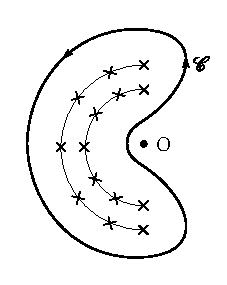
\includegraphics{figures/fig61-7.4.eps}
\caption{}
\label{chap1:fig7.4}
\end{figure}
\noindent
are acceptable. Hence solutions can be obtained which are similar to the case $k=0$ but with double the number of terms. The solution for perfect reflection (regular at the shoreline) is obtained from the path $\mathscr{C}$ chosen as in Fig. 7.4. This time there is an essential singularity at $\zeta =0$ which must be excluded, otherwise unacceptable solutions in positive powers of $x$ and $y$ would be obtained. This choice of $\mathscr{C}$ satisfies the rotation requirement noted after equation \eqref{chap7:eq7.70}. The rotation requirement excludes paths going between the poles on either semicircle, but an alternative is still to take a path enclosing only one or the other semicircle. However such choices give the same solution as the one shown, with an additional numerical factor.

When $x=y=0$, the integrands in \eqref{chap7:eq7.75} are asymptotic to $1/\zeta$ as $\zeta\to\infty$. Therefore
$$
S(0,0)=1
$$\pageoriginale
as before.

\subsection*{\bf Behavior as $x\to\infty$}.

The asymptotic behavior as $x\to\infty$ is given by the four poles with $\mathscr{R}\zeta=0$, namely
\begin{equation}
\zeta=\pm i\frac{\lambda+\ell}{2},\;\zeta=\pm i \frac{\lambda-\ell}{2}. \tag{7.77}\label{chap7:eq7.77}
\end{equation}

We then have, after some simplification of the factors in the residues, 
\begin{equation}
S(x,y)\sim\frac{1}{2CD}\left\{\frac{1+(-1)^N\rho^N}{1-\rho}\right\} e^{i\ell x+\lambda y}+c.c.,\tag{7.78}\label{chap7:eq7.78}
\end{equation}
where
\begin{align}
D&=(1-w)\,(1-w^2)\ldots\left(1-w^{N-1}\right),\;w=e^{\pi i/N}, \tag{7.79}\label{chap7:eq7.79}\\
C&= (1-\rho w)\,(1-\rho^2)\ldots\left(1-\rho w^{N-1}\right),\;\rho= \frac{\lambda-\ell}{\lambda+\ell}.\tag{7.80}\label{chap7:eq7.80}
\end{align}

Combined with \eqref{chap7:eq7.58}, we see that \eqref{chap7:eq7.78} represents the perfect reflection of an incoming oblique wave with direction $(-\ell,k)$.

The coefficient $D$ arose in the case of normal incidence $(\rho=0)$ and was found in \eqref{chap7:eq7.36} to be 
\begin{equation}
D=N^{1/2}e^{-\pi i\frac{N-1}{4}}\tag{7.81}\label{chap7:eq7.81}
\end{equation}

We can find $|C|$ by an argument similar to the one used for $D$. We consider
\begin{align*}
CC^* &= (1-\rho w)\ldots\left(1-\rho w^{N-1}\right)\,\left(1-\rho w^{-1}\right) \ldots \left(1-\rho w^{-(n-1)}\right)\\
&= \underset{W\to 1}{\lim}(W-\rho w)\ldots \left(W-\rho w^{N-1}\right)\, \left(W-\rho w^{-1}\right)\ldots\left(W-\rho w^{(N-1)}\right)\\
&= \underset{W\to 1}{\lim }\frac{W^{2N}-\rho^{2N}}{(W-\rho)\,(W+\rho)}\\
&= \frac{1-\rho^{2N}}{1-\rho^2}\tag{7.82}\label{chap7:eq7.82}
\end{align*}\pageoriginale

There appears to be no simplified expression for $\arg C$. However, we have simplified the expression for the amplitude; \eqref{chap7:eq7.78} becomes 
\begin{gather}
S(x,y)\sim\frac{1}{2N^{1/2}}\left\{\frac{1+(-1)^N\rho^N}{1-(-1)^N\rho^N}. \frac{1+\rho}{1-\rho}\right\}^{1/2} e^{i\ell x+\lambda y+i\alpha}+c.c., \tag{7.83}\label{chap7:eq7.83}\\
\intertext{where}
\alpha = - \arg C+\pi(N-1)/4.\tag{7.84}\label{chap7:eq7.84}
\end{gather}

When $\rho\to 1$, there is a surprising difference in the behavior of the amplitude depending on whether $N$ is odd or even. It is perhaps best viewed by renormalizing the solution so that the amplitude of the incoming wave is unity and the amplitude at the shoreline becomes
\begin{equation}
a_0=N^{1/2}\left\{\frac{1-(-1)^N\rho^N}{1+(-1)^N\rho^N}\;\frac{1-\rho}{1+\rho} \right\}^{1/2}.\tag{7.85}\label{chap7:eq7.85}
\end{equation}

When $N$ is even $a_0\to 0$ as $\rho\to 1$, whereas it remains finite for $N$ odd. However, in this limit $C\to D$ so that 
$$
\alpha\to\pi(N-1)/2.
$$

When $N$ is even, $2\alpha$ is an odd multiple of $\pi$ so the incoming and reflected wave are exactly out of phase in the limit and cancel. When $N$ is odd, $2\alpha$ is an even multiple of $\pi$ so the incoming and reflected waves reinforce. Related to this is the fact (seen below) that when $N$ is odd a new edge wave mode appears, and just when it appears the more usual exponential decay is absent.

Neverthless,\pageoriginale the behavior is quite strange. For large values of $N$ the corresponding changes in $\beta$ are small and one would not expect rapid changes in behavior as $N$ oscillates between odd and even values.

\subsection*{\bf Singular solutions}.

As in the case of normal incidence, solutions with zero or partial reflection may be obtained by taking the path of integration in \eqref{chap7:eq7.75} to be similar to the paths $\mathscr{C}_1, \mathscr{C}_2$ in Fig. \eqref{chap7:eq7.3}. In this case, because of the essential singularity at $\zeta =0$, they must go into the origin with $\mathscr{R}\zeta <0$. 

\section{Edge waves, $0<\lambda <k$}\label{chap7:sec7.7}

For $\lambda$ in the range $(0,k)$, if we set 
\begin{equation}
\lambda=k\sin\mu, \; 0<\mu <\pi/2,\tag{7.86}\label{chap7:eq7.86}
\end{equation}
the roots of the quadratic in \eqref{chap7:eq7.74} are given by
\begin{equation}
(A)\quad \frac{k}{2}w^n e^{i\mu},\quad (B)\quad -\frac{k}{2}w^n e^{-i\mu}. \tag{7.87}\label{chap7:eq7.87}
\end{equation}

These lie on two different semicircles of the {\bf same} circle as indicated in Fig. \ref{chap7:eq7.5}.

Now these are poles of the integrals in \eqref{chap7:eq7.75}. Those with $\mathscr{R}\zeta <0$ would lead to exponentials with positive exponents in $x$ and are unacceptable (since we require bounded solutions as $x\to\infty$). Therefore, the contributions of the poles with $\mathscr{R}\zeta >0$ must cancel between the two integrals in \eqref{chap7:eq7.75}. This will only be possible for 
\begin{figure}[H]
\centering
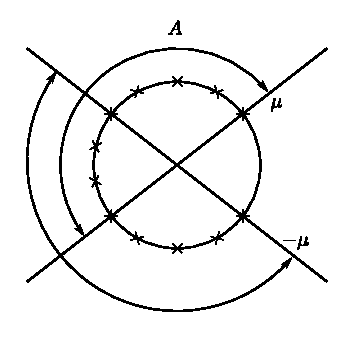
\includegraphics{figures/fig61-7.5.eps}
\caption{}
\label{chap1:fig7.5}
\end{figure}\pageoriginale
\noindent
certain values of $\lambda$, and leads to the restriction of $\lambda$ to a discrete set of values: the point spectrum.

To carry out the details, we take the same contour $\mathscr{C}$ as before, but deform it into the 
\begin{figure}[H]
\centering
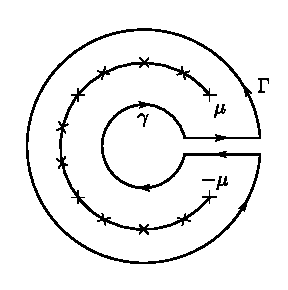
\includegraphics{figures/fig61-7.6.eps}
\caption{}
\label{chap1:fig7.6}
\end{figure}
\noindent
two circles $\Gamma$ and $\gamma$ as shown in Fig. 7.6. Furthermore, the substitution of $\zeta=k^2/4\xi$ in the integrals on $\gamma$ converts them into integrals on $\Gamma$. When this is carried through, and pairs of integrals combined, we have 
\begin{align*}
S(x,y) &=\frac{1}{4\pi i}\int\limits_\Gamma\frac{\zeta^{N-1}\left\{\zeta^N+\left( \frac{k^2}{4\zeta}\right)^N\right\}}{Q_1\cdots Q_N} e^{\left(\zeta+\frac{k^2} {4\zeta}\right)x+i\left(\zeta-\frac{k^2}{4\zeta}\right)y}\,d\zeta\\
&+ \frac{1}{4\pi i}\int\limits_\Gamma \frac{\zeta^{N-1}\left\{\zeta^N+\left( \frac{k^2}{4\zeta}\right)^N\right\}}{Q_0\cdots Q_{N-1}} e^{\left(\zeta+\frac{k^2} {4\zeta}\right)x-i\left(\zeta-\frac{k^2}{4\zeta}\right)y}\,d\zeta. \tag{7.88}\label{chap7:eq7.88}
\end{align*}

It\pageoriginale should be especially noted that the final form fits with the original \eqref{chap7:eq7.69}, but for a different function $f(\zeta)$. Thus there is a very important lack of uniqueness in the solution of the functional relation \eqref{chap7:eq7.72}. However, the solutions for $S(x,y)$ are the same; the change of $f(\zeta)$ is compensated for by the change in contour form $\mathscr{C}$ to $\Gamma$.

Now the requirement that poles with $\mathscr{R}\zeta >0$ do not contribute is easily obtained. The factor in the numerator of \eqref{chap7:eq7.88},
\begin{equation}
\zeta^N+\left(\frac{k^2}{4\zeta}\right)^N\tag{7.89}\label{chap7:eq7.89}
\end{equation}
vanishes at points
\begin{equation}
\zeta=\frac{k^2}{2} e^{\pi i\frac{2q+1}{2N}},\; q=\quad\text{integer}. \tag{7.90}\label{chap7:eq7.90}
\end{equation}

These zeros are equally spaced around the circle in Fig.7.5, with angles $\pi/N$ between them. If $\mu$ is tuned so that these zeros lie on the poles there will be no singularities in the parts of $A$ and $B$ where $A$ and $B$ do not overlap, and this includes all those with $\mathscr{R}\zeta >0$. Where $A$ and $B$ do overlap, the double poles will be converted to single poles and provide non-zero contributions. Thus, the requirement is 
\begin{equation}
\mu=\frac{2p+1}{2N}\pi\tag{7.91}\label{chap7:eq7.91}
\end{equation}
for some integer $p$. For $\lambda$ in \eqref{chap7:eq7.86} we have
\begin{equation}
\lambda_p=k\sin(2p+1)\frac{\pi}{2N}=k\sin(2p+1)\beta. \tag{7.92}\label{chap7:eq7.92}
\end{equation}
where $(2p+1)\beta<\pi/2$. This is the result quoted in \eqref{chap7:eq7.67}.

If\pageoriginale we denote the modified $f(\zeta)$ that appears in \eqref{chap7:eq7.88} by $f_1(\zeta)$, we have 
$$
f_1(\zeta)=\frac{\zeta^{2N}+\left(\frac{k^2}{4}\right)^N}{\zeta Q_1(\zeta)\cdots Q_N(\zeta)}.
$$

For $\lambda=\lambda_p$ as given in \eqref{chap7:eq7.91}-\eqref{chap7:eq7.92}, the cancellation of appropriate factors can be carried through and we are left with 
\begin{equation}
f_1(\zeta)=\frac{1}{\zeta}\;\frac{\zeta-\frac{k}{2} e^{-(2p-1)i\beta}}{\zeta+ \frac{k}{2} e^{-(2p-1)i\beta}}\ldots \frac{\zeta-\frac{k}{2} e^{(2p+1)i\beta}} {\zeta+\frac{k}{2} e^{(2p+1)i\beta}}.\tag{7.93}\label{chap7:eq7.93}
\end{equation}

Here the relation $\beta =\pi/2N$ has been used to eliminate $N$ in favour of $\beta$. {\bf In this form}, \eqref{chap7:eq7.93} is valid for any $\beta$, and is no longer limited to submultiples of $\pi/2$. So the edge wave solutions $S(x,y)$ can be extended to all $\beta$ using \eqref{chap7:eq7.93}. The first one, 
\begin{align*}
& p=0, \lambda_0=k\sin\beta,\\
&f_1(\zeta)=\frac{1}{\zeta}\;\frac{\zeta-\frac{k}{2} e^{i\beta}}{\zeta+ \frac{k}{2}e^{i\beta}},\tag{7.94}\label{chap7:eq7.94}
\end{align*}
leads to the Stokes solution \eqref{chap7:eq7.65}.

As regards the direct strategy for finding \eqref{chap7:eq7.93} from \eqref{chap7:eq7.72}, we note that \eqref{chap7:eq7.72}, with $\lambda=k\sin \mu$, can be written 
\begin{equation}
f_1(\zeta)=e^{2i\beta}\frac{\left(\zeta-\frac{k}{2}e^{i\mu}\right)\;\left(\zeta+ \frac{k}{2}e^{-i\mu}\right)}{\left(\zeta+\frac{k}{2}e^{i\mu}\right)\;\left(\zeta- \frac{k}{2}e^{-i\mu}\right)}f_1\left(\zeta e^{2i\beta}\right). \tag{7.95}\label{chap7:eq7.95}
\end{equation}

When\pageoriginale $\mu=(2p+1)\beta$, one would have to note how an appropriate number of iterations and some re-arrangement allows the solution to be picked off. For example, in the Stokes case $\mu=\beta$, \eqref{chap7:eq7.95} can be re-written 
\begin{equation}
f_1(\zeta)=\frac{\zeta e^{2i\beta}}{\zeta}\;\left(\frac{\zeta-\frac{k}{2} e^{i\beta}}{\zeta+\frac{k}{2} e^{i\beta}}\right)\;\left(\frac{\zeta 2^{2i\beta}+ \frac{k}{2}e^{i\beta}}{\zeta e^{2i\beta}-\frac{k}{2}e^{i\beta}}\right)f_1\left( \zeta e^{2i\beta}\right).\tag{7.96}\label{chap7:eq7.96}
\end{equation}

Then one checks that \eqref{chap7:eq7.94} is a solution. But this may not have been easy to see in advance, especially for higher $p$.

